
\subsubsection{O que são requisitos}

Em suma, um requisito determina uma capacidade ou condição que deve ser satisfeita pelo sistema. Ou seja, um requisito especifica funções executadas pelo sistema ou uma qualidades que ele deve ter.

Os requisitos podem se relacionar de diversas maneiras:  Contêm (\textit{containment}), Deriva(\textit{derive}), Satisfaz(\textit{satisfy}), Verifica(\textit{verify}), Rastreia(\textit{trace}) e Copia(\textit{copy}). De maneira geral, existe uma hierarquia de entre os requisitos.

Em SysML, há uma expansão em relação ao UML, em que requisitos podem ter relacionamentos não só entre si , mas com elementos de design, analises, casos de testes, também. 


\subsubsection{Estrutura dos diagramas de requisitos}
O diagrama de requisitos representa os requisitos e as relações entre eles seu objetivo é permitir uma visualização da hierarquia dos requisitos na especificação de projeto. 

A ideia é organizar os requisitos de alto nível e baixo nível, de maneira a deixar clara sua diferenciação, mas mantendo suas ligações. 

 Ligações de "contenção" são representado por uma ligação solida com uma cruz dentro de uma circunferência, as outras são relações seguem a conexão de associação detalhada em 2.2.1.

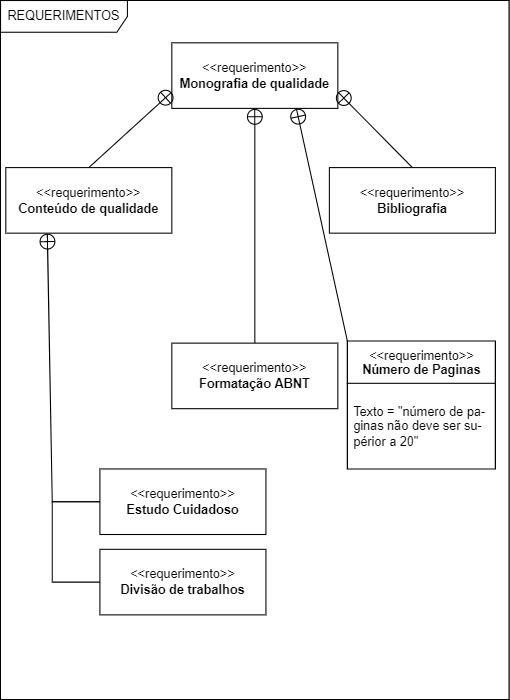
\includegraphics[width=\textwidth/2,height=\textheight,keepaspectratio]{figures/diagrama de requistos exemplo 1.png}
